% Options for packages loaded elsewhere
\PassOptionsToPackage{unicode}{hyperref}
\PassOptionsToPackage{hyphens}{url}
\PassOptionsToPackage{dvipsnames,svgnames,x11names}{xcolor}
%
\documentclass[
  letterpaper,
  DIV=11,
  numbers=noendperiod,
  oneside]{scrartcl}

\usepackage{amsmath,amssymb}
\usepackage{iftex}
\ifPDFTeX
  \usepackage[T1]{fontenc}
  \usepackage[utf8]{inputenc}
  \usepackage{textcomp} % provide euro and other symbols
\else % if luatex or xetex
  \usepackage{unicode-math}
  \defaultfontfeatures{Scale=MatchLowercase}
  \defaultfontfeatures[\rmfamily]{Ligatures=TeX,Scale=1}
\fi
\usepackage{lmodern}
\ifPDFTeX\else  
    % xetex/luatex font selection
\fi
% Use upquote if available, for straight quotes in verbatim environments
\IfFileExists{upquote.sty}{\usepackage{upquote}}{}
\IfFileExists{microtype.sty}{% use microtype if available
  \usepackage[]{microtype}
  \UseMicrotypeSet[protrusion]{basicmath} % disable protrusion for tt fonts
}{}
\makeatletter
\@ifundefined{KOMAClassName}{% if non-KOMA class
  \IfFileExists{parskip.sty}{%
    \usepackage{parskip}
  }{% else
    \setlength{\parindent}{0pt}
    \setlength{\parskip}{6pt plus 2pt minus 1pt}}
}{% if KOMA class
  \KOMAoptions{parskip=half}}
\makeatother
\usepackage{xcolor}
\usepackage[left=1in,marginparwidth=2.0666666666667in,textwidth=4.1333333333333in,marginparsep=0.3in]{geometry}
\setlength{\emergencystretch}{3em} % prevent overfull lines
\setcounter{secnumdepth}{5}
% Make \paragraph and \subparagraph free-standing
\ifx\paragraph\undefined\else
  \let\oldparagraph\paragraph
  \renewcommand{\paragraph}[1]{\oldparagraph{#1}\mbox{}}
\fi
\ifx\subparagraph\undefined\else
  \let\oldsubparagraph\subparagraph
  \renewcommand{\subparagraph}[1]{\oldsubparagraph{#1}\mbox{}}
\fi

\usepackage{color}
\usepackage{fancyvrb}
\newcommand{\VerbBar}{|}
\newcommand{\VERB}{\Verb[commandchars=\\\{\}]}
\DefineVerbatimEnvironment{Highlighting}{Verbatim}{commandchars=\\\{\}}
% Add ',fontsize=\small' for more characters per line
\usepackage{framed}
\definecolor{shadecolor}{RGB}{241,243,245}
\newenvironment{Shaded}{\begin{snugshade}}{\end{snugshade}}
\newcommand{\AlertTok}[1]{\textcolor[rgb]{0.68,0.00,0.00}{#1}}
\newcommand{\AnnotationTok}[1]{\textcolor[rgb]{0.37,0.37,0.37}{#1}}
\newcommand{\AttributeTok}[1]{\textcolor[rgb]{0.40,0.45,0.13}{#1}}
\newcommand{\BaseNTok}[1]{\textcolor[rgb]{0.68,0.00,0.00}{#1}}
\newcommand{\BuiltInTok}[1]{\textcolor[rgb]{0.00,0.23,0.31}{#1}}
\newcommand{\CharTok}[1]{\textcolor[rgb]{0.13,0.47,0.30}{#1}}
\newcommand{\CommentTok}[1]{\textcolor[rgb]{0.37,0.37,0.37}{#1}}
\newcommand{\CommentVarTok}[1]{\textcolor[rgb]{0.37,0.37,0.37}{\textit{#1}}}
\newcommand{\ConstantTok}[1]{\textcolor[rgb]{0.56,0.35,0.01}{#1}}
\newcommand{\ControlFlowTok}[1]{\textcolor[rgb]{0.00,0.23,0.31}{#1}}
\newcommand{\DataTypeTok}[1]{\textcolor[rgb]{0.68,0.00,0.00}{#1}}
\newcommand{\DecValTok}[1]{\textcolor[rgb]{0.68,0.00,0.00}{#1}}
\newcommand{\DocumentationTok}[1]{\textcolor[rgb]{0.37,0.37,0.37}{\textit{#1}}}
\newcommand{\ErrorTok}[1]{\textcolor[rgb]{0.68,0.00,0.00}{#1}}
\newcommand{\ExtensionTok}[1]{\textcolor[rgb]{0.00,0.23,0.31}{#1}}
\newcommand{\FloatTok}[1]{\textcolor[rgb]{0.68,0.00,0.00}{#1}}
\newcommand{\FunctionTok}[1]{\textcolor[rgb]{0.28,0.35,0.67}{#1}}
\newcommand{\ImportTok}[1]{\textcolor[rgb]{0.00,0.46,0.62}{#1}}
\newcommand{\InformationTok}[1]{\textcolor[rgb]{0.37,0.37,0.37}{#1}}
\newcommand{\KeywordTok}[1]{\textcolor[rgb]{0.00,0.23,0.31}{#1}}
\newcommand{\NormalTok}[1]{\textcolor[rgb]{0.00,0.23,0.31}{#1}}
\newcommand{\OperatorTok}[1]{\textcolor[rgb]{0.37,0.37,0.37}{#1}}
\newcommand{\OtherTok}[1]{\textcolor[rgb]{0.00,0.23,0.31}{#1}}
\newcommand{\PreprocessorTok}[1]{\textcolor[rgb]{0.68,0.00,0.00}{#1}}
\newcommand{\RegionMarkerTok}[1]{\textcolor[rgb]{0.00,0.23,0.31}{#1}}
\newcommand{\SpecialCharTok}[1]{\textcolor[rgb]{0.37,0.37,0.37}{#1}}
\newcommand{\SpecialStringTok}[1]{\textcolor[rgb]{0.13,0.47,0.30}{#1}}
\newcommand{\StringTok}[1]{\textcolor[rgb]{0.13,0.47,0.30}{#1}}
\newcommand{\VariableTok}[1]{\textcolor[rgb]{0.07,0.07,0.07}{#1}}
\newcommand{\VerbatimStringTok}[1]{\textcolor[rgb]{0.13,0.47,0.30}{#1}}
\newcommand{\WarningTok}[1]{\textcolor[rgb]{0.37,0.37,0.37}{\textit{#1}}}

\providecommand{\tightlist}{%
  \setlength{\itemsep}{0pt}\setlength{\parskip}{0pt}}\usepackage{longtable,booktabs,array}
\usepackage{calc} % for calculating minipage widths
% Correct order of tables after \paragraph or \subparagraph
\usepackage{etoolbox}
\makeatletter
\patchcmd\longtable{\par}{\if@noskipsec\mbox{}\fi\par}{}{}
\makeatother
% Allow footnotes in longtable head/foot
\IfFileExists{footnotehyper.sty}{\usepackage{footnotehyper}}{\usepackage{footnote}}
\makesavenoteenv{longtable}
\usepackage{graphicx}
\makeatletter
\def\maxwidth{\ifdim\Gin@nat@width>\linewidth\linewidth\else\Gin@nat@width\fi}
\def\maxheight{\ifdim\Gin@nat@height>\textheight\textheight\else\Gin@nat@height\fi}
\makeatother
% Scale images if necessary, so that they will not overflow the page
% margins by default, and it is still possible to overwrite the defaults
% using explicit options in \includegraphics[width, height, ...]{}
\setkeys{Gin}{width=\maxwidth,height=\maxheight,keepaspectratio}
% Set default figure placement to htbp
\makeatletter
\def\fps@figure{htbp}
\makeatother

\KOMAoption{captions}{tableheading}
\makeatletter
\@ifpackageloaded{caption}{}{\usepackage{caption}}
\AtBeginDocument{%
\ifdefined\contentsname
  \renewcommand*\contentsname{Table of contents}
\else
  \newcommand\contentsname{Table of contents}
\fi
\ifdefined\listfigurename
  \renewcommand*\listfigurename{List of Figures}
\else
  \newcommand\listfigurename{List of Figures}
\fi
\ifdefined\listtablename
  \renewcommand*\listtablename{List of Tables}
\else
  \newcommand\listtablename{List of Tables}
\fi
\ifdefined\figurename
  \renewcommand*\figurename{Figure}
\else
  \newcommand\figurename{Figure}
\fi
\ifdefined\tablename
  \renewcommand*\tablename{Table}
\else
  \newcommand\tablename{Table}
\fi
}
\@ifpackageloaded{float}{}{\usepackage{float}}
\floatstyle{ruled}
\@ifundefined{c@chapter}{\newfloat{codelisting}{h}{lop}}{\newfloat{codelisting}{h}{lop}[chapter]}
\floatname{codelisting}{Listing}
\newcommand*\listoflistings{\listof{codelisting}{List of Listings}}
\makeatother
\makeatletter
\makeatother
\makeatletter
\@ifpackageloaded{caption}{}{\usepackage{caption}}
\@ifpackageloaded{subcaption}{}{\usepackage{subcaption}}
\makeatother
\makeatletter
\@ifpackageloaded{sidenotes}{}{\usepackage{sidenotes}}
\@ifpackageloaded{marginnote}{}{\usepackage{marginnote}}
\makeatother
\ifLuaTeX
  \usepackage{selnolig}  % disable illegal ligatures
\fi
\IfFileExists{bookmark.sty}{\usepackage{bookmark}}{\usepackage{hyperref}}
\IfFileExists{xurl.sty}{\usepackage{xurl}}{} % add URL line breaks if available
\urlstyle{same} % disable monospaced font for URLs
\hypersetup{
  pdftitle={Setting up a minimal neovim environment for data science code development},
  pdfauthor={Ronald (Ryy) Glenn Thomas},
  colorlinks=true,
  linkcolor={blue},
  filecolor={Maroon},
  citecolor={Blue},
  urlcolor={Blue},
  pdfcreator={LaTeX via pandoc}}

\title{Setting up a minimal neovim environment for data science code
development}
\usepackage{etoolbox}
\makeatletter
\providecommand{\subtitle}[1]{% add subtitle to \maketitle
  \apptocmd{\@title}{\par {\large #1 \par}}{}{}
}
\makeatother
\subtitle{A neovim IDE for R, Python, and Julia}
\author{Ronald (Ryy) Glenn Thomas}
\date{2023-07-18}

\begin{document}
\maketitle
\renewcommand*\contentsname{Table of contents}
{
\hypersetup{linkcolor=}
\setcounter{tocdepth}{3}
\tableofcontents
}
\marginnote{\begin{footnotesize}

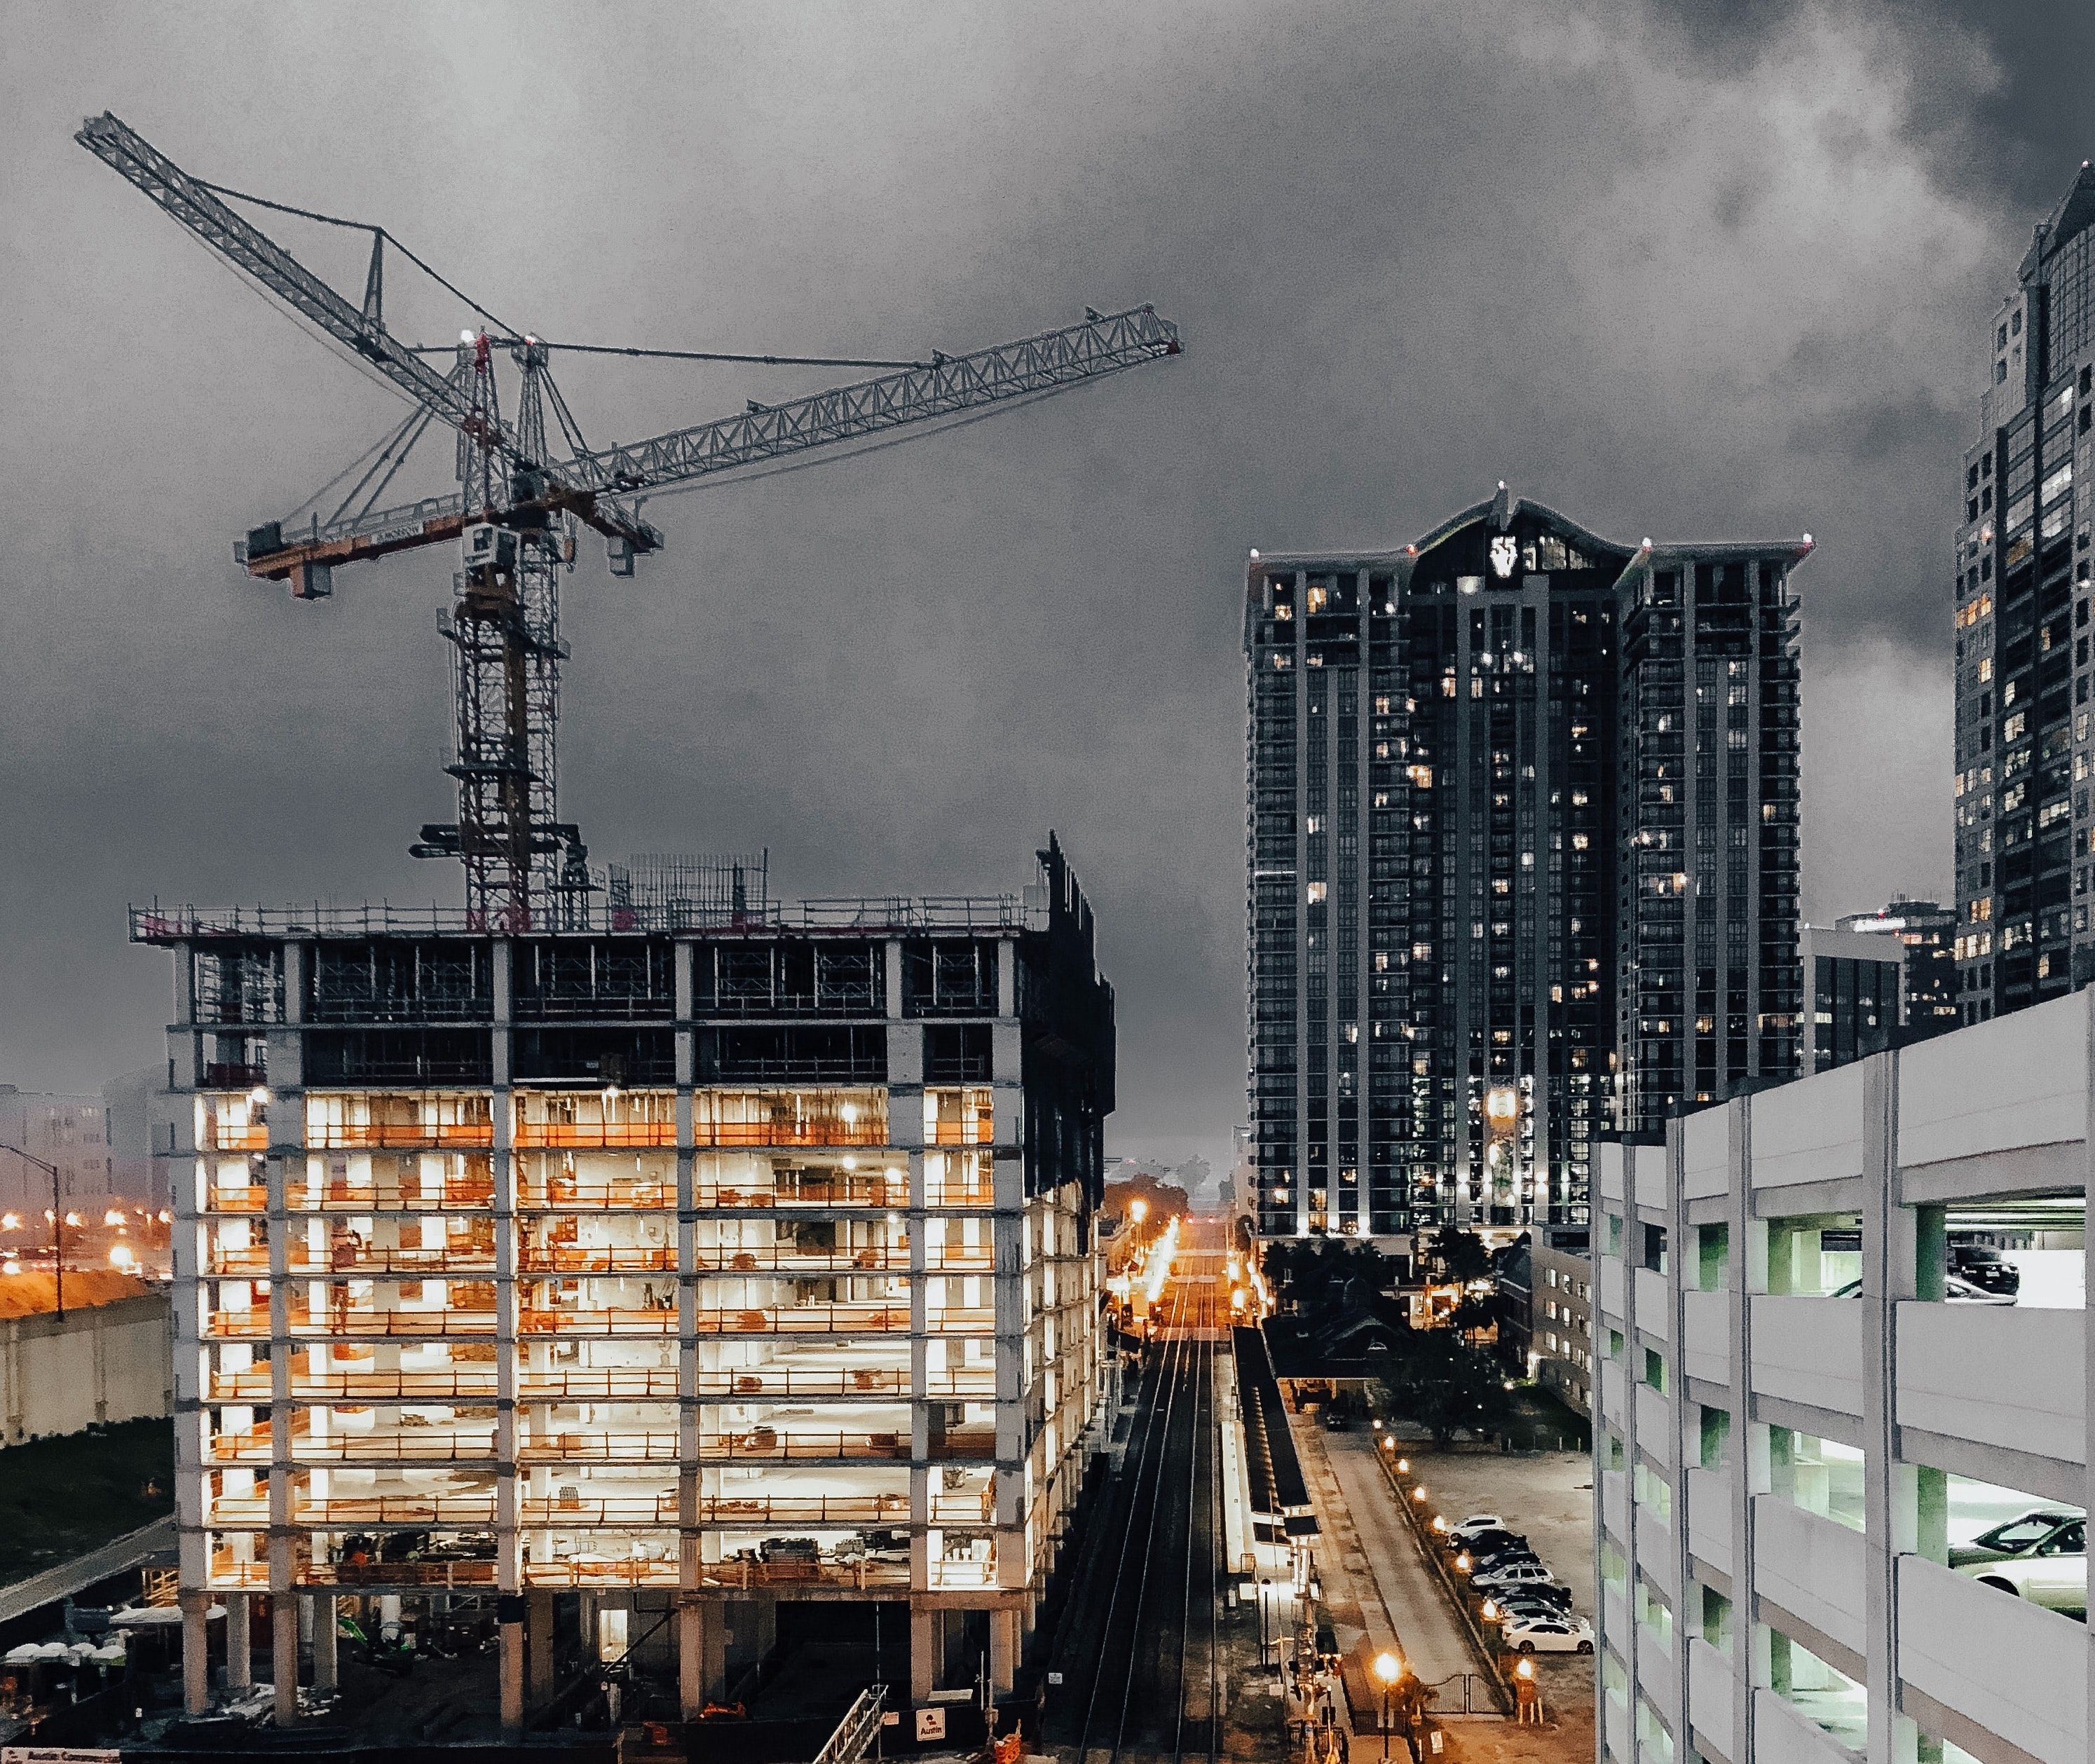
\includegraphics{img/crane.jpg} Photo by Nathan Waters on Unsplash

\end{footnotesize}}

\section{Introduction}\label{introduction}

Neovim (a fork of Vim) is a text editor that has several advantages for
data science code development. One of the main attractions is that it is
open source and has a number of useful plugins to facilitate working on
R, python, and julia code. Also, its modal, keyboard-centric system
allows text and code manipulation at potentially far greater speed than
conventional, mouse-centric, systems.

In this post we describe both a minimal, yet functional setup, as well
as a more extensive setup utilizing several of the newest neovim-only
plugins, for neovim to allow IDE style code editing and REPL interaction
for the three primary data science coding tools: R, Python, and Julia.

Our presentation here is for a Macos environment. Appendix one contains
required adjustments for a ubuntu linux environment.

\section{Install the latest stable version of
neovim.}\label{install-the-latest-stable-version-of-neovim.}

With minimal effort we can install both the terminal and GUI versions of
neovim. The simplist approach is to use homebrew:

\begin{Shaded}
\begin{Highlighting}[]
\OperatorTok{\textgreater{}}\NormalTok{ brew }\FunctionTok{install}\NormalTok{ neovim neovim{-}qt}
\end{Highlighting}
\end{Shaded}

Set up convenience aliases in \texttt{zsh}.

\begin{Shaded}
\begin{Highlighting}[]
\OperatorTok{\textgreater{}}\NormalTok{ alias }\ExtensionTok{ng}\NormalTok{ = neovim{-}qt}
\OperatorTok{\textgreater{}}\NormalTok{ alias }\ExtensionTok{nt}\NormalTok{ = neovim}
\end{Highlighting}
\end{Shaded}

(mnemonic: the \texttt{t} in \texttt{nt} is for terminal, the \texttt{g}
in \texttt{ng} is for GUI)

\section{Configure neovim}\label{configure-neovim}

The standard location for \texttt{neovim} configuration files on
``unix-like'' systems is \texttt{\textasciitilde{}/.config/nvim}. The
main config file is either init.vim (VimL) or init.lua (Lua). In this
post we'll focus on lua based configuration.

Specifically, the following code block creates an \texttt{nvim}
subdirectory under \texttt{\textasciitilde{}/.config} and initialize a
configuration file \texttt{init.lua}.

Here is the file hierarchy we'll construct. In fact all the code could
be bundled into the \texttt{init.lua} file, but this approach is clearer
and cleaner.

\begin{Shaded}
\begin{Highlighting}[]
\BuiltInTok{.}
\KeywordTok{|}\ExtensionTok{{-}{-}}\NormalTok{ ginit.vim}
\KeywordTok{|}\ExtensionTok{{-}{-}}\NormalTok{ init.lua}
\KeywordTok{|}\ExtensionTok{{-}{-}}\NormalTok{ lazy{-}lock.json}
\KeywordTok{|}\ExtensionTok{{-}{-}}\NormalTok{ lua}
\KeywordTok{|}   \KeywordTok{|}\ExtensionTok{{-}{-}}\NormalTok{ basics.lua}
\KeywordTok{|}   \KeywordTok{|}\ExtensionTok{{-}{-}}\NormalTok{ leap{-}config.lua}
\KeywordTok{|}   \KeywordTok{|}\ExtensionTok{{-}{-}}\NormalTok{ nvim{-}R{-}config.lua}
\KeywordTok{|}   \KeywordTok{|}\ExtensionTok{{-}{-}}\NormalTok{ nvim{-}cmp{-}config.lua}
\KeywordTok{|}   \KeywordTok{|}\ExtensionTok{{-}{-}}\NormalTok{ nvim{-}telescope{-}config.lua}
\KeywordTok{|}   \KeywordTok{|}\ExtensionTok{{-}{-}}\NormalTok{ nvim{-}tree{-}config.lua}
\KeywordTok{|}   \KeywordTok{\textasciigrave{}}\ExtensionTok{{-}{-}}\NormalTok{ treesitter{-}config.lua}
\KeywordTok{|}\ExtensionTok{{-}{-}}\NormalTok{ my\_snippets}
\KeywordTok{|}   \KeywordTok{|}\ExtensionTok{{-}{-}}\NormalTok{ all.snippets}
\KeywordTok{|}   \KeywordTok{|}\ExtensionTok{{-}{-}}\NormalTok{ giles.tex.snipppets}
\KeywordTok{|}   \KeywordTok{|}\ExtensionTok{{-}{-}}\NormalTok{ mail.snippets}
\KeywordTok{|}   \KeywordTok{|}\ExtensionTok{{-}{-}}\NormalTok{ r.snippets}
\KeywordTok{|}   \KeywordTok{|}\ExtensionTok{{-}{-}}\NormalTok{ rmd.snippets}
\KeywordTok{|}   \KeywordTok{|}\ExtensionTok{{-}{-}}\NormalTok{ snippets.snippets}
\KeywordTok{|}   \KeywordTok{|}\ExtensionTok{{-}{-}}\NormalTok{ tex.snippets}
\KeywordTok{|}   \KeywordTok{|}\ExtensionTok{{-}{-}}\NormalTok{ text.snippets}
\KeywordTok{|}   \KeywordTok{\textasciigrave{}}\AttributeTok{{-}{-}}\NormalTok{ txt.snippets}
\KeywordTok{|}\ExtensionTok{{-}{-}}\NormalTok{ spell}
\KeywordTok{|}   \KeywordTok{|}\ExtensionTok{{-}{-}}\NormalTok{ en.utf{-}8.add}
\KeywordTok{|}   \KeywordTok{\textasciigrave{}}\ExtensionTok{{-}{-}}\NormalTok{ en.utf{-}8.add.spl}
\end{Highlighting}
\end{Shaded}

To install the \texttt{lazy} plugin manager

\begin{Shaded}
\begin{Highlighting}[]
\FunctionTok{git}\NormalTok{ clone https://github.com/folke/lazy.nvim.git }\DataTypeTok{\textbackslash{}}
\NormalTok{   \textasciitilde{}/.local/share/nvim/lazy/lazy.nvim}
\end{Highlighting}
\end{Shaded}

Add the following code to \texttt{init.lua} list the plugins needed to
be installed from \texttt{github} and ``feed'' them to \texttt{Lazy} for
installation.

Nvim-R, Leap, UltiSnips, and vimtex need additional configuration. The
required code is contained in bespoke files under the \texttt{lua}
directory.

\begin{Shaded}
\begin{Highlighting}[]



\ExtensionTok{vim.g.mapleader}\NormalTok{ = }\StringTok{","}
\ExtensionTok{vim.g.maplocalleader}\NormalTok{ = }\StringTok{" "}
\ExtensionTok{vim.opt.rtp:prepend}\ErrorTok{(}\StringTok{"\textasciitilde{}/.local/share/nvim/lazy/lazy.nvim"}\KeywordTok{)}
\ExtensionTok{require}\ErrorTok{(}\StringTok{\textquotesingle{}plugins\textquotesingle{}}\KeywordTok{)}
\ExtensionTok{require}\ErrorTok{(}\StringTok{\textquotesingle{}basics\textquotesingle{}}\KeywordTok{)}
\ExtensionTok{require}\ErrorTok{(}\StringTok{\textquotesingle{}nvim{-}tree{-}config\textquotesingle{}}\KeywordTok{)}
\ExtensionTok{require}\ErrorTok{(}\StringTok{\textquotesingle{}nvim{-}R{-}config\textquotesingle{}}\KeywordTok{)}
\ExtensionTok{require}\ErrorTok{(}\StringTok{\textquotesingle{}nvim{-}telescope{-}config\textquotesingle{}}\KeywordTok{)}
\ExtensionTok{require}\ErrorTok{(}\StringTok{\textquotesingle{}leap\textquotesingle{}}\KeywordTok{)}\FunctionTok{.add\_default\_mappings()}
\ExtensionTok{require}\ErrorTok{(}\StringTok{\textquotesingle{}leap{-}config\textquotesingle{}}\KeywordTok{)}
\ExtensionTok{require}\ErrorTok{(}\StringTok{\textquotesingle{}lualine\textquotesingle{}}\KeywordTok{)}\FunctionTok{.setup()}
\end{Highlighting}
\end{Shaded}

List of plugins

\begin{Shaded}
\begin{Highlighting}[]






\ExtensionTok{require}\ErrorTok{(}\StringTok{\textquotesingle{}lazy\textquotesingle{}}\KeywordTok{)}\ExtensionTok{.setup}\ErrorTok{(}\KeywordTok{\{}
\ExtensionTok{{-}{-}}
\ExtensionTok{{-}{-}minimal}\NormalTok{ data science setup}
\ExtensionTok{{-}{-}}
\StringTok{\textquotesingle{}jalvesaq/Nvim{-}R\textquotesingle{}}\ExtensionTok{,}
\StringTok{\textquotesingle{}lervag/vimtex\textquotesingle{}}\ExtensionTok{,}
\StringTok{\textquotesingle{}SirVer/ultisnips\textquotesingle{}}\ExtensionTok{,}
\StringTok{\textquotesingle{}jalvesaq/vimcmdline\textquotesingle{}}\ExtensionTok{,}
\ExtensionTok{{-}{-}}
\ExtensionTok{{-}{-}optional}\NormalTok{ utilities}
\ExtensionTok{{-}{-}}
\StringTok{"nvim{-}lualine/lualine.nvim"}\ExtensionTok{,}
\StringTok{"bluz71/vim{-}moonfly{-}colors"}\ExtensionTok{,}
\StringTok{\textquotesingle{}junegunn/vim{-}peekaboo\textquotesingle{}}\ExtensionTok{,}
\StringTok{\textquotesingle{}tpope/vim{-}commentary\textquotesingle{}}\ExtensionTok{,}
\StringTok{\textquotesingle{}francoiscabrol/ranger.vim\textquotesingle{}}\ExtensionTok{,}
\StringTok{\textquotesingle{}machakann/vim{-}highlightedyank\textquotesingle{}}\ExtensionTok{,}
\StringTok{\textquotesingle{}tpope/vim{-}surround\textquotesingle{}}\ExtensionTok{,}
\StringTok{\textquotesingle{}ggandor/leap.nvim\textquotesingle{}}\ExtensionTok{,}
\ExtensionTok{{-}{-}}
\ExtensionTok{{-}{-}neovim}\NormalTok{ specific}
\StringTok{\textquotesingle{}nvim{-}lua/plenary.nvim\textquotesingle{}}\ExtensionTok{,}
\StringTok{\textquotesingle{}nvim{-}tree/nvim{-}web{-}devicons\textquotesingle{}}\ExtensionTok{,}
\StringTok{\textquotesingle{}nvim{-}tree/nvim{-}tree.lua\textquotesingle{}}\ExtensionTok{,}
\StringTok{\textquotesingle{}nvim{-}telescope/telescope.nvim\textquotesingle{}}\ExtensionTok{,}
\StringTok{\textquotesingle{}nvim{-}treesitter/nvim{-}treesitter\textquotesingle{}}\ExtensionTok{,}
\StringTok{\textquotesingle{}neovim/nvim{-}lspconfig\textquotesingle{}}\ExtensionTok{,}
\KeywordTok{\})}

\end{Highlighting}
\end{Shaded}

\section{plugin discussions}\label{plugin-discussions}

\begin{verbatim}


# basics
```sh






local map = vim.keymap.set
local opts = {noremap = true}
vim.cmd([[
"    paste registers into terminal
tnoremap <expr> <C-R> '<C-\><C-N>"'.nr2char(getchar()).'pi'
set background=dark
colorscheme moonfly
let $FZF_DEFAULT_COMMAND = 'rg --files --hidden'
set completeopt=menu,menuone,noinsert,noselect
set number relativenumber
set textwidth=80
set cursorline
set clipboard=unnamed
set iskeyword-=_ 
set hlsearch   
set splitright
set hidden   
set incsearch    
set noswapfile
set showmatch
set ignorecase
set smartcase
set gdefault
filetype plugin on
set encoding=utf-8
set nobackup
set nowritebackup
set updatetime=300
set signcolumn=yes
set colorcolumn=80
set timeoutlen=1000 ttimeoutlen=10
let g:UltiSnipsSnippetDirectories = ['~/.config/nvim/my_snippets']
let g:UltiSnipsExpandTrigger="<tab>"
let g:UltiSnipsJumpForwardTrigger="<c-j>"
let g:UltiSnipsJumpBackwardTrigger="<c-k>"
nnoremap <leader>U <Cmd>call UltiSnips#RefreshSnippets()<CR>

autocmd BufWinEnter,WinEnter term://* startinsert
"autocmd TermOpen * exec "normal! i"
]])
map('n', ':', ';', opts)
map('n', ';', ':', opts)
map('n', '<leader>u',':UltiSnipsEdit<cr>', opts)
map('n', '<leader>U','<Cmd>call UltiSnips#RefreshSnippets()<cr>', opts)
map('n', '<localleader><localleader>','<C-d>', opts)
map('n', '-','$', opts)
map('n', '<leader>w','vipgq', opts)
map('n', '<leader>v',':edit ~/.config/nvim/init.lua<cr>', opts)
map('n', '<leader>n',':edit ~/.config/nvim/lua/basics.lua<cr>', opts)
map('n', '<leader>a','ggVG', opts)
map('n', '<leader>t',':tab split<cr>', opts)
map('n', '<leader>y',':vert sb3<cr>', opts)
map('n', '<leader>0',':ls!<CR>:b<Space>', opts)
map('n', '<leader><leader>','<C-w>w', opts)
map('n', '<leader>1','<C-w>:b1<cr>', opts)
map('n', '<leader>2','<C-w>:b2<cr>', opts)
map('n', '<leader>3','<C-w>:b3<cr>', opts)
map('t',  'ZZ', "q('yes')<CR>", opts)
map('t',  'ZQ', "q('no')<CR>", opts)
map('v',  '-', '$', opts)
map('t',  '<leader>0','<C-\\><C-n><C-w>:ls!<cr>:b<Space>', opts)
map('t',  '<Escape>','<C-\\><C-n>', opts)
map('t',  ',,','<C-\\><C-n><C-w>w', opts)
map('i',  '<Esc>', '<Esc>`^', opts)
\end{verbatim}

\section{Set up R}\label{set-up-r}

\begin{Shaded}
\begin{Highlighting}[]






\ExtensionTok{vim.cmd}\ErrorTok{(}\KeywordTok{[[}
\NormalTok{iabb }\OtherTok{\textless{}}\NormalTok{buffer}\ErrorTok{\textgreater{}} \ErrorTok{x} \ExtensionTok{\%}\OperatorTok{\textgreater{}}\NormalTok{\%}
\ExtensionTok{iabb} \OperatorTok{\textless{}}\NormalTok{buffer}\OperatorTok{\textgreater{}}\NormalTok{ z \%in\% }
\BuiltInTok{let} \VariableTok{R\_auto\_start} \OperatorTok{=} \DecValTok{2}
\BuiltInTok{let} \VariableTok{R\_enable\_comment} \OperatorTok{=} \DecValTok{1}
\BuiltInTok{let} \VariableTok{R\_hl\_term} \OperatorTok{=} \DecValTok{0}
\BuiltInTok{let} \VariableTok{R\_clear\_line} \OperatorTok{=} \DecValTok{1}
\BuiltInTok{let} \VariableTok{R\_pdfviewer} \OperatorTok{=} \StringTok{"zathura"} 
\BuiltInTok{let} \VariableTok{R\_assign} \OperatorTok{=} \DecValTok{2}
\BuiltInTok{let} \VariableTok{R\_latexcmd} \OperatorTok{=} \OperatorTok{[}\StringTok{\textquotesingle{}xelatex\textquotesingle{}}\OperatorTok{]}
\ExtensionTok{augroup}\NormalTok{ rmarkdown}
\ExtensionTok{autocmd!}
\ExtensionTok{autocmd}\NormalTok{ FileType rmd,r nnoremap }\OperatorTok{\textless{}}\NormalTok{buffer}\OperatorTok{\textgreater{}} \OperatorTok{\textless{}}\NormalTok{CR}\OperatorTok{\textgreater{}}\NormalTok{  :call SendLineToR}\ErrorTok{(}\StringTok{"down"}\KeywordTok{)}\OperatorTok{\textless{}}\NormalTok{CR}\OperatorTok{\textgreater{}}
\ExtensionTok{autocmd}\NormalTok{ FileType rmd,r nnoremap }\OperatorTok{\textless{}}\NormalTok{buffer}\OperatorTok{\textgreater{}} \OperatorTok{\textless{}}\NormalTok{space}\OperatorTok{\textgreater{}}\StringTok{\textquotesingle{} :call RMakeRmd("default")\textless{}cr\textgreater{}}
\StringTok{autocmd FileType rmd,r noremap \textless{}space\textgreater{}i :call RAction("dim")\textless{}cr\textgreater{}}
\StringTok{autocmd FileType rmd,r noremap \textless{}space\textgreater{}h :call RAction("head")\textless{}cr\textgreater{}}
\StringTok{autocmd FileType rmd,r noremap \textless{}space\textgreater{}p :call RAction("print")\textless{}cr\textgreater{}}
\StringTok{autocmd FileType rmd,r noremap \textless{}space\textgreater{}q :call RAction("length")\textless{}cr\textgreater{}}
\StringTok{autocmd FileType rmd,r noremap \textless{}space\textgreater{}n :call RAction("nvim.names")\textless{}cr\textgreater{}}
\StringTok{autocmd FileType rmd,r vmap \textless{}buffer\textgreater{} \textless{}CR\textgreater{} \textless{}localleader\textgreater{}sd}
\StringTok{autocmd FileType rmd,r nmap \textless{}buffer\textgreater{} \textless{}space\textgreater{}j \textless{}localleader\textgreater{}gn}
\StringTok{autocmd FileType rmd,r nmap \textless{}buffer\textgreater{} \textless{}space\textgreater{}k \textless{}localleader\textgreater{}gN}
\StringTok{autocmd FileType rmd,r nmap \textless{}buffer\textgreater{} \textless{}space\textgreater{}l \textless{}localleader\textgreater{}cd}
\StringTok{augroup END}
\StringTok{]])}






\end{Highlighting}
\end{Shaded}

\section{Appendix Ubuntu tweaks}\label{appendix-ubuntu-tweaks}



\end{document}
